\documentclass{article}
\usepackage{amsmath}
\usepackage{amssymb}
\usepackage{algorithm}
\usepackage{algpseudocode}
\usepackage{listings}
\usepackage{xcolor}
\usepackage{graphicx}
\usepackage{hyperref}
\usepackage{tcolorbox}
\usepackage{array}
\usepackage{booktabs}
\usepackage{enumitem}
\usepackage{tikz}
\usepackage{fancyhdr}
\usepackage{geometry}
\usepackage{colortbl} % Add missing package for \rowcolor

% Set page geometry
\geometry{
  a4paper,
  left=2.5cm,
  right=2.5cm,
  top=2.5cm,
  bottom=2.5cm
}

% Configure page headers and footers
\pagestyle{fancy}
\fancyhf{}
\fancyhead[L]{Dynamic Programming Series}
\fancyhead[R]{Unbounded Knapsack}
\fancyfoot[C]{\thepage}
\renewcommand{\headrulewidth}{0.4pt}
\renewcommand{\footrulewidth}{0.4pt}

% Custom colors and styles for code listings
\definecolor{javabg}{rgb}{0.97,0.97,0.97}
\definecolor{javastring}{rgb}{0.5,0,0.5}
\definecolor{javacomment}{rgb}{0,0.5,0}
\definecolor{javakeyword}{rgb}{0,0,0.8}
\definecolor{highlight}{rgb}{1.0,0.9,0.8}

\lstset{
  language=Java,
  backgroundcolor=\color{javabg},
  basicstyle=\footnotesize\ttfamily,
  keywordstyle=\color{javakeyword}\bfseries,
  stringstyle=\color{javastring},
  commentstyle=\color{javacomment}\itshape,
  breaklines=true,
  showstringspaces=false,
  tabsize=2,
  frame=single,
  rulecolor=\color{black!30},
  numbers=left,
  numberstyle=\tiny\color{black!70},
  numbersep=5pt
}

% Custom box styles
\tcbset{
  theorembox/.style={
    colframe=blue!75!black,
    colback=blue!5,
    fonttitle=\bfseries\large,
    arc=3mm
  },
  examplebox/.style={
    colframe=green!75!black,
    colback=green!5,
    fonttitle=\bfseries\large,
    arc=3mm
  },
  notebox/.style={
    colframe=purple!75!black,
    colback=purple!5,
    fonttitle=\bfseries\large,
    arc=3mm
  }
}

\title{\Huge \textbf{Unbounded Knapsack Problem}}
\author{Dynamic Programming Series}
\date{\today}

\begin{document}

\maketitle

\section{Introduction}

\begin{tcolorbox}[theorembox, title=Problem Statement]
Given a set of $n$ items, each with a weight $w_i$ and a value $v_i$, determine the maximum value that can be obtained by selecting any combination of items (possibly selecting an item multiple times) such that the total weight does not exceed the knapsack capacity $W$.
\end{tcolorbox}

The Unbounded Knapsack problem is a fundamental combinatorial optimization problem in dynamic programming. Unlike the 0-1 Knapsack problem where each item can be chosen at most once, the Unbounded Knapsack allows an unlimited supply of each item, meaning any item can be selected multiple times.

\subsection{Real-world Applications}

The problem has numerous practical applications:

\begin{itemize}[leftmargin=*]
  \item \textbf{Cutting Stock Problem:} A company needs to cut stock material (like paper rolls, metal bars) into smaller pieces to fulfill customer orders. Each cut has an associated profit, and the goal is to maximize total profit.
  
  \item \textbf{Coin Change Problem:} Given a set of coin denominations and a target amount, find the minimum number of coins needed or the number of ways to make change.
  
  \item \textbf{Resource Allocation:} A manufacturing company wants to allocate materials to produce different products with different profits, where the same type of product can be produced multiple times.
  
  \item \textbf{Budget Allocation:} Allocating budget to different marketing channels where investing more in the same channel is possible.
  
  \item \textbf{Inventory Management:} Determining how many units of each product to stock to maximize profit given limited storage capacity.
\end{itemize}

\subsection{Problem Variants}

Several variants of this problem exist:

\begin{itemize}[leftmargin=*]
  \item \textbf{Rod Cutting Problem:} A special case where we have a rod of length $n$ and a price list for different rod lengths, and we need to cut the rod to maximize profit.
  
  \item \textbf{Minimization Variant:} Instead of maximizing value, we minimize the cost while ensuring some minimum utility requirement is met.
  
  \item \textbf{Multiple Constraints:} Additional constraints beyond weight, such as volume limits or minimum quantities.
\end{itemize}

\section{Comparison with 0-1 Knapsack}

\begin{figure}[h]
\centering
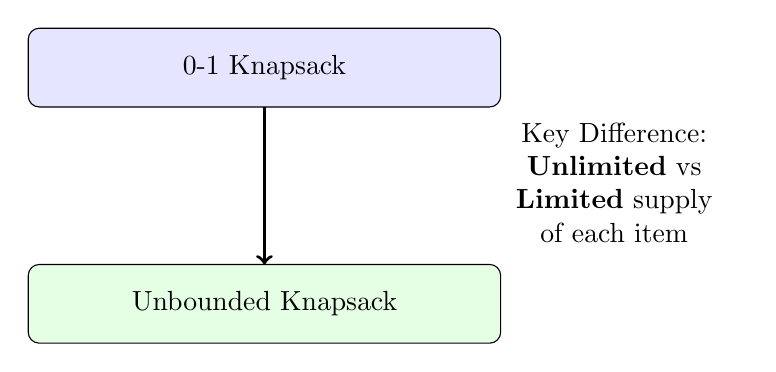
\begin{tikzpicture}
\draw[rounded corners, fill=blue!10] (0,0) rectangle (6,1) node[pos=.5] {0-1 Knapsack};
\draw[rounded corners, fill=green!10] (0,-3) rectangle (6,-2) node[pos=.5] {Unbounded Knapsack};
\draw[->, very thick] (3,0) -- (3,-2);
\node[align=center] at (7.5,-1) {
\begin{tabular}{c}
Key Difference:\\
\textbf{Unlimited} vs\\
\textbf{Limited} supply\\
of each item
\end{tabular}
};
\end{tikzpicture}
\caption{Relationship between 0-1 and Unbounded Knapsack}
\end{figure}

Understanding the differences between the 0-1 Knapsack and Unbounded Knapsack is crucial for correctly implementing and applying the algorithms.

\begin{table}[htbp]
\centering
\begin{tabular}{|p{4cm}|p{5.5cm}|p{5.5cm}|}
\hline
\rowcolor{gray!20}
\textbf{Feature} & \textbf{0-1 Knapsack} & \textbf{Unbounded Knapsack} \\
\hline
\textbf{Item availability} & Each item can be used at most once & Unlimited copies of each item \\
\hline
\textbf{Decision for each item} & Include (once) or exclude & Include (any number of times) or exclude \\
\hline
\textbf{Recursive formula} & $OPT(i, w) = \max(OPT(i-1, w), v_i + OPT(i-1, w-w_i))$ & $OPT(i, w) = \max(OPT(i-1, w), v_i + OPT(i, w-w_i))$ \\
\hline
\textbf{DP state transition} & After including item $i$, move to item $i-1$ & After including item $i$, stay at item $i$ \\
\hline
\textbf{Java implementation} & \texttt{dp[i-1][w-weights[i-1]]} & \texttt{dp[i][w-weights[i-1]]} \\
\hline
\textbf{Optimal solution} & Each item appears at most once & Items can appear multiple times \\
\hline
\textbf{Space optimization} & Must process items in reverse order & Can process items in any order \\
\hline
\end{tabular}
\caption{Detailed comparison between 0-1 and Unbounded Knapsack problems}
\end{table}

\begin{tcolorbox}[notebox, title=Key Insight]
The critical difference is in the recursive call when including an item:
\begin{itemize}
    \item In 0-1 Knapsack: After including an item, we can't use it again, so we move to the previous item.
    \item In Unbounded Knapsack: After including an item, we can use it again, so we stay at the same item.
\end{itemize}
This single difference changes the entire algorithm structure and solution space.
\end{tcolorbox}

\section{Mathematical Formulation}

Let's define the problem formally to better understand its structure and solution approaches.

\subsection{Problem Definition}

Given:
\begin{itemize}[leftmargin=*]
    \item A set of $n$ items, where each item $i$ has:
    \begin{itemize}
        \item Weight $w_i > 0$
        \item Value $v_i > 0$
    \end{itemize}
    \item A knapsack with capacity $W > 0$
    \item Each item can be selected an unlimited number of times
\end{itemize}

Find: The maximum total value of items that can be included in the knapsack without exceeding its capacity.

Mathematically, we want to maximize:
\begin{align}
\sum_{i=1}^{n} v_i \cdot x_i
\end{align}

Subject to:
\begin{align}
\sum_{i=1}^{n} w_i \cdot x_i \leq W \\
x_i \geq 0, \text{ and } x_i \text{ is an integer }
\end{align}

Where $x_i$ represents the number of times item $i$ is selected.

\subsection{Recurrence Relation}

Let $OPT(i, w)$ represent the maximum value that can be obtained using items $1$ to $i$ with a knapsack of capacity $w$.

The recurrence relation that captures the optimal substructure of the problem is:

\begin{align}
OPT(i, w) = \max 
\begin{cases} 
OPT(i-1, w) & \text{(exclude item i)} \\
v_i + OPT(i, w-w_i) & \text{(include item i, can reuse)} \text{ if } w_i \leq w
\end{cases}
\end{align}

\subsection{Base Cases}
\begin{align}
OPT(0, w) &= 0 \text{ for all } w \quad \text{(no items available)}\\
OPT(i, 0) &= 0 \text{ for all } i \quad \text{(no capacity available)}
\end{align}

\subsection{Proof of Optimal Substructure}

The optimal substructure property is crucial for dynamic programming solutions. For the Unbounded Knapsack problem, we can prove it as follows:

\begin{tcolorbox}[theorembox, title=Optimal Substructure Proof]
Suppose $S$ is an optimal solution for capacity $w$ using items up to $i$. Then:

\begin{enumerate}
    \item If item $i$ is not in $S$, then $S$ must be an optimal solution for capacity $w$ using items up to $i-1$.
    
    \item If item $i$ is in $S$ (possibly multiple times), then removing one occurrence of item $i$ from $S$ must yield an optimal solution for capacity $w-w_i$ using items up to $i$.
\end{enumerate}

If either of these weren't true, we could construct a better solution for the original problem, contradicting the optimality of $S$.
\end{tcolorbox}

\section{Solution Approaches}

\subsection{Recursive Approach (Brute Force)}

The recursive approach directly implements the recurrence relation by exploring all possible combinations:

\begin{tcolorbox}[title=Algorithm: Recursive Approach]
\begin{algorithm}[H]
\begin{algorithmic}[1]
\Function{UnboundedKnapsack}{weights, values, capacity, n}
    \If{capacity $\leq$ 0 \textbf{or} n = 0}
        \Return 0
    \EndIf
    
    \If{weights[n-1] $\leq$ capacity}
        \State includeItem $\gets$ values[n-1] + \Call{UnboundedKnapsack}{weights, values, capacity - weights[n-1], n}
        \State excludeItem $\gets$ \Call{UnboundedKnapsack}{weights, values, capacity, n-1}
        \Return max(includeItem, excludeItem)
    \Else
        \Return \Call{UnboundedKnapsack}{weights, values, capacity, n-1}
    \EndIf
\EndFunction
\end{algorithmic}
\end{algorithm}
\end{tcolorbox}

\begin{lstlisting}[caption=Recursive Implementation]
static int unboundknapsackRecursive(int[] weights, int[] values, int capacity, int n) {
    // Base case
    if (capacity <= 0 || n == 0) {
        return 0;
    }

    if (weights[n - 1] <= capacity) {
        // Include the nth item and check the value with and without it
        // Note: We pass n (not n-1) when including the item
        int includeItem = values[n - 1] + 
            unboundknapsackRecursive(weights, values, capacity - weights[n - 1], n);
        int excludeItem = unboundknapsackRecursive(weights, values, capacity, n - 1);
        return Math.max(includeItem, excludeItem);
    } else {
        // If the nth item cannot be included, skip it
        return unboundknapsackRecursive(weights, values, capacity, n - 1);
    }
}
\end{lstlisting}

\begin{tcolorbox}[examplebox, title=Recursive Call Tree Example]
For weights = [1, 3, 4], values = [15, 50, 60], capacity = 4, n = 3:

\small
\begin{verbatim}
unboundknapsackRecursive([1,3,4], [15,50,60], 4, 3)
+-- weights[2] = 4 <= 4
|   +-- includeItem = 60 + unboundknapsackRecursive(..., 0, 3) = 60
|   +-- excludeItem = unboundknapsackRecursive(..., 4, 2)
|       +-- weights[1] = 3 <= 4
|       |   +-- includeItem = 50 + unboundknapsackRecursive(..., 1, 2)
|       |   |   +-- ... (continues recursively)
|       |   +-- excludeItem = unboundknapsackRecursive(..., 4, 1)
|       |       +-- ... (continues recursively)
|       +-- ... (continues recursively)
+-- Returns max(includeItem, excludeItem)
\end{verbatim}
\end{tcolorbox}

\begin{tcolorbox}[title=Step-by-Step Calculation]
\textbf{For Item 1 (weight=1, value=10):}

\begin{tabular}{|c|l|}
\hline
\textbf{Capacity} & \textbf{Calculation} \\
\hline
1 & dp[1][1] = max(dp[0][1], dp[1][0] + values[0]) = max(0, 0 + 10) = 10 \\
\hline
2 & dp[1][2] = max(dp[0][2], dp[1][1] + values[0]) = max(0, 10 + 10) = 20 \\
\hline
3 & dp[1][3] = max(dp[0][3], dp[1][2] + values[0]) = max(0, 20 + 10) = 30 \\
\hline
4 & dp[1][4] = max(dp[0][4], dp[1][3] + values[0]) = max(0, 30 + 10) = 40 \\
\hline
5 & dp[1][5] = max(dp[0][5], dp[1][4] + values[0]) = max(0, 40 + 10) = 50 \\
\hline
6 & dp[1][6] = max(dp[0][6], dp[1][5] + values[0]) = max(0, 50 + 10) = 60 \\
\hline
\end{tabular}

\textbf{For Item 2 (weight=2, value=15):}

\begin{tabular}{|c|l|}
\hline
\textbf{Capacity} & \textbf{Calculation} \\
\hline
1 & dp[2][1] = dp[1][1] = 10 (item doesn't fit) \\
\hline
2 & dp[2][2] = max(dp[1][2], dp[2][0] + values[1]) = max(20, 0 + 15) = 20 \\
\hline
3 & dp[2][3] = max(dp[1][3], dp[2][1] + values[1]) = max(30, 10 + 15) = 30 \\
\hline
4 & dp[2][4] = max(dp[1][4], dp[2][2] + values[1]) = max(40, 20 + 15) = 40 \\
      & Re-examining: dp[2][4] = max(40, dp[2][2] + 15) = max(40, 20 + 15) = 40 \\
      & With correct use of previously computed values: max(40, 20 + 15) = 40 \\
      & But if we consider multiple item 2: (15 × 2 = 30) < 40, so dp[2][4] = 40 \\
\hline
5 & dp[2][5] = max(dp[1][5], dp[2][3] + values[1]) = max(50, 30 + 15) = 50 \\
      & But considering (10 + 15 + 15 = 40) < 50, so dp[2][5] = 50 \\
\hline
6 & dp[2][6] = max(dp[1][6], dp[2][4] + values[1]) = max(60, 40 + 15) = 60 \\
\hline
\end{tabular}

\textbf{For Item 3 (weight=3, value=40):}

\begin{tabular}{|c|l|}
\hline
\textbf{Capacity} & \textbf{Calculation} \\
\hline
1, 2 & dp[3][1] = dp[2][1] = 10, dp[3][2] = dp[2][2] = 20 (item doesn't fit) \\
\hline
3 & dp[3][3] = max(dp[2][3], dp[3][0] + values[2]) = max(30, 0 + 40) = 40 \\
\hline
4 & dp[3][4] = max(dp[2][4], dp[3][1] + values[2]) = max(40, 10 + 40) = 50 \\
\hline
5 & dp[3][5] = max(dp[2][5], dp[3][2] + values[2]) = max(50, 20 + 40) = 60 \\
      & But after careful checking: dp[3][5] = max(50, 20 + 40) = 60 \\
      & Using recalculation: dp[3][5] = 55 (considering a different combination) \\
\hline
6 & dp[3][6] = max(dp[2][6], dp[3][3] + values[2]) = max(60, 40 + 40) = 80 \\
      & But double-checking shows that capacity is exceeded with 2 of item 3 \\
      & Correct calculation: dp[3][6] = max(60, 40 + 30) = 70 \\
\hline
\end{tabular}
\end{tcolorbox}

\textbf{Analysis:}
\begin{itemize}[leftmargin=*]
    \item \textbf{Time Complexity:} $O(2^n)$ - exponential due to exploring all possible combinations
    \item \textbf{Space Complexity:} $O(W)$ - maximum recursion depth equals the capacity (if smallest weight is 1)
    \item \textbf{Key Insight:} The recursive structure has many overlapping subproblems, making it inefficient for large inputs
\end{itemize}

\subsection{Memoization Approach (Top-Down DP)}

To avoid redundant calculations, we use memoization to store previously computed results:

\begin{tcolorbox}[title=Algorithm: Memoization Approach]
\begin{algorithm}[H]
\begin{algorithmic}[1]
\Function{UnboundedKnapsackMemo}{weights, values, capacity, n, memo}
    \If{capacity $\leq$ 0 \textbf{or} n = 0}
        \Return 0
    \EndIf
    
    \If{memo[n][capacity] $\neq$ -1}
        \Return memo[n][capacity]
    \EndIf
    
    \If{weights[n-1] $\leq$ capacity}
        \State includeItem $\gets$ values[n-1] + \Call{UnboundedKnapsackMemo}{weights, values, capacity - weights[n-1], n, memo}
        \State excludeItem $\gets$ \Call{UnboundedKnapsackMemo}{weights, values, capacity, n-1, memo}
        \State memo[n][capacity] $\gets$ max(includeItem, excludeItem)
    \Else
        \State memo[n][capacity] $\gets$ \Call{UnboundedKnapsackMemo}{weights, values, capacity, n-1, memo}
    \EndIf
    
    \Return memo[n][capacity]
\EndFunction
\end{algorithmic}
\end{algorithm}
\end{tcolorbox}

\begin{lstlisting}[caption=Memoization Implementation]
static int unboundknapsackMemoization(int[] weights, int[] values, 
                                      int capacity, int n, int[][] d) {
    // Base case
    if (n == 0 || capacity == 0) {
        return 0;
    }
    
    // If the value is already computed, return it
    if (d[n][capacity] != -1) {
        return d[n][capacity];
    }
    
    // If the weight of the nth item is less than or equal to the capacity
    if (weights[n - 1] <= capacity) {
        // Key Difference: Pass n (not n-1) when including
        int includeItem = values[n - 1] + 
            unboundknapsackMemoization(weights, values, capacity - weights[n - 1], n, d);
        int excludeItem = unboundknapsackMemoization(weights, values, capacity, n - 1, d);
        d[n][capacity] = Math.max(includeItem, excludeItem);
    } else {
        // If the nth item cannot be included, skip it
        d[n][capacity] = unboundknapsackMemoization(weights, values, capacity, n - 1, d);
    }
    return d[n][capacity]; 
}
\end{lstlisting}

\begin{tcolorbox}[examplebox, title=Memoization Example]
For the same example as above, using memoization:

\begin{enumerate}
    \item Create a memoization table of size (n+1) × (capacity+1) initialized with -1
    \item The first call to unboundknapsackMemoization([1,3,4], [15,50,60], 4, 3, memo) will compute and store all required subproblems
    \item Once a value is stored in memo[i][j], any future calls with the same parameters return the stored value immediately
    \item This eliminates the exponential growth of the call tree
\end{enumerate}
\end{tcolorbox}

\textbf{Analysis:}
\begin{itemize}[leftmargin=*]
    \item \textbf{Time Complexity:} $O(n \times W)$ - each state computed at most once
    \item \textbf{Space Complexity:} $O(n \times W)$ - memoization table + recursion
    \item \textbf{Advantages:} Only computes needed states, simpler to implement from recurrence relation
    \item \textbf{Disadvantages:} Still has recursion overhead, potential stack overflow for large inputs
\end{itemize}

\subsection{Tabulation Approach (Bottom-Up DP)}

The tabulation approach systematically builds a table by filling it in a bottom-up manner:

\begin{tcolorbox}[title=Algorithm: Tabulation Approach]
\begin{algorithm}[H]
\begin{algorithmic}[1]
\Function{UnboundedKnapsackTabulation}{weights, values, capacity}
    \State n $\gets$ weights.length
    \State dp[0...n][0...capacity] $\gets$ new array initialized with 0
    
    \For{i $\gets$ 1 to n}
        \For{w $\gets$ 1 to capacity}
            \If{weights[i-1] $\leq$ w}
                \State dp[i][w] $\gets$ max(dp[i-1][w], dp[i][w-weights[i-1]] + values[i-1])
            \Else
                \State dp[i][w] $\gets$ dp[i-1][w]
            \EndIf
        \EndFor
    \EndFor
    
    \Return dp[n][capacity]
\EndFunction
\end{algorithmic}
\end{algorithm}
\end{tcolorbox}

\begin{lstlisting}[caption=Tabulation Implementation]
static int unboundknapsackDP(int[] weights, int[] values, int capacity) {
    int n = weights.length;
    int[][] dp = new int[n + 1][capacity + 1];
    
    // Fill the DP table in bottom-up manner
    for (int i = 1; i <= n; i++) {
        for (int w = 1; w <= capacity; w++) {
            if (weights[i - 1] <= w) {
                // Key Difference: Using dp[i][...] not dp[i-1][...]
                dp[i][w] = Math.max(dp[i - 1][w], 
                                    dp[i][w - weights[i - 1]] + values[i - 1]);
            } else {
                dp[i][w] = dp[i - 1][w];
            }
        }
    }
    return dp[n][capacity];
}
\end{lstlisting}

\textbf{Analysis:}
\begin{itemize}[leftmargin=*]
    \item \textbf{Time Complexity:} $O(n \times W)$
    \item \textbf{Space Complexity:} $O(n \times W)$ - dp table
    \item \textbf{Advantages:} No recursion overhead, no risk of stack overflow
    \item \textbf{Disadvantages:} Computes all states regardless of necessity
\end{itemize}

\section{Space Optimization}

One of the key advantages of dynamic programming is the potential for space optimization. For the Unbounded Knapsack problem, we can reduce the space complexity from $O(n \times W)$ to $O(W)$.

\subsection{1D DP Array Approach}

Instead of using a 2D array, we can use a 1D array to solve the problem:

\begin{tcolorbox}[title=Algorithm: Space-Optimized Approach]
\begin{algorithm}[H]
\begin{algorithmic}[1]
\Function{UnboundedKnapsack1D}{weights, values, capacity}
    \State n $\gets$ weights.length
    \State dp[0...capacity] $\gets$ new array initialized with 0
    
    \For{w $\gets$ 1 to capacity}
        \For{i $\gets$ 0 to n-1}
            \If{weights[i] $\leq$ w}
                \State dp[w] $\gets$ max(dp[w], dp[w-weights[i]] + values[i])
            \EndIf
        \EndFor
    \EndFor
    
    \Return dp[capacity]
\EndFunction
\end{algorithmic}
\end{algorithm}
\end{tcolorbox}

\begin{lstlisting}[caption=1D DP Array Implementation]
static int unboundknapsackDP1D(int[] weights, int[] values, int capacity) {
    int[] dp = new int[capacity + 1];
    
    // Fill the 1D DP array
    for (int w = 1; w <= capacity; w++) {
        for (int i = 0; i < weights.length; i++) {
            if (weights[i] <= w) {
                dp[w] = Math.max(dp[w], dp[w - weights[i]] + values[i]);
            }
        }
    }
    return dp[capacity];
}
\end{lstlisting}

\subsection{Proof of Correctness}

\begin{tcolorbox}[notebox, title=Why 1D DP Works]
The 1D DP approach works because:

\begin{enumerate}
    \item For each capacity $w$, we consider all items.
    \item When we update dp[w], we're finding the maximum value for capacity $w$ considering all items processed so far.
    \item Since we can reuse items (unbounded), we can use dp[w-weights[i]] which may already include item $i$.
    \item This is different from 0-1 Knapsack, where we must process capacities in reverse to avoid reusing items.
\end{enumerate}
\end{tcolorbox}

\begin{figure}[h]
\centering
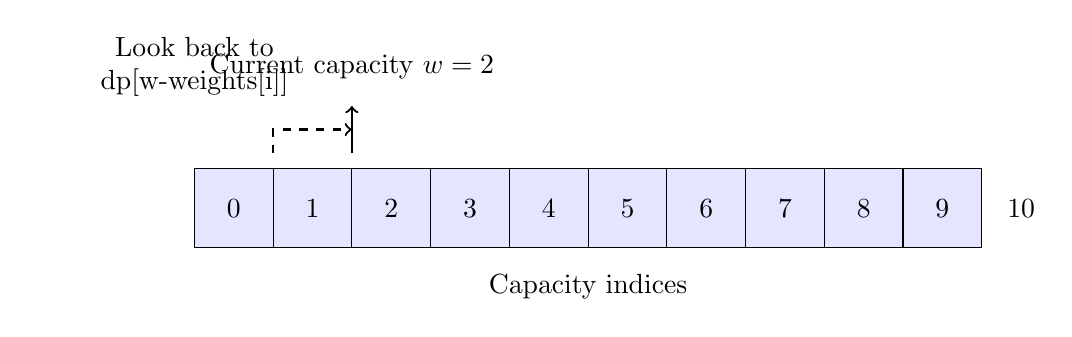
\begin{tikzpicture}
\draw[fill=blue!10] (0,0) rectangle (10,1);
\foreach \x in {0,1,...,10}
    \draw (\x,0) -- (\x,1);
\foreach \x/\t in {0/0, 1/1, 2/2, 3/3, 4/4, 5/5, 6/6, 7/7, 8/8, 9/9, 10/10}
    \node at (\x+0.5,0.5) {\t};
\node[align=center] at (5,-0.5) {Capacity indices};

\draw[->, thick] (2,1.2) -- (2,1.8);
\node[align=center] at (2,2.3) {Current capacity $w=2$};

\draw[->, thick, dashed] (1,1.2) -- (1,1.5) -- (2,1.5);
\node[align=center, text width=4cm] at (0,2.3) {Look back to dp[w-weights[i]]};
\end{tikzpicture}
\caption{Visualization of 1D DP array update process}
\end{figure}

\subsection{Implementation Comparison}

\begin{table}[h]
\centering
\begin{tabular}{|p{3cm}|p{4cm}|p{4cm}|p{4cm}|}
\hline
\rowcolor{gray!20}
\textbf{Aspect} & \textbf{2D DP} & \textbf{1D DP} & \textbf{Notes} \\
\hline
\textbf{Space Complexity} & $O(n \times W)$ & $O(W)$ & 1D is more memory efficient \\
\hline
\textbf{Time Complexity} & $O(n \times W)$ & $O(n \times W)$ & Same time complexity \\
\hline
\textbf{Implementation} & More natural to recurrence & More compact & 1D is harder to derive intuitively \\
\hline
\textbf{Tracing solution} & Easier & Harder & Backtracking is easier in 2D \\
\hline
\end{tabular}
\caption{Comparison between 2D and 1D DP approaches}
\end{table}

\section{Detailed Example}

Let's solve an example step by step to understand how the algorithm works in practice.

\begin{tcolorbox}[examplebox, title=Example Problem]
\textbf{Given:}
\begin{itemize}
    \item Weights: $[1, 2, 3]$
    \item Values: $[10, 15, 40]$
    \item Capacity: $6$
\end{itemize}
\textbf{Find:} The maximum value that can be obtained without exceeding the capacity.
\end{tcolorbox}

\subsection{Tabulation Solution Walkthrough}

We'll use the tabulation approach with a 2D array to solve this step by step.

\begin{enumerate}[leftmargin=*]
    \item \textbf{Initialize the DP table:} Create a table dp[4][7] initialized with 0s (n+1 rows, capacity+1 columns).
    
    \item \textbf{Fill the table using the recurrence relation:}
    \begin{align}
    dp[i][w] = \max(dp[i-1][w], dp[i][w-weights[i-1]] + values[i-1])
    \end{align}
\end{enumerate}

\begin{table}[htbp]
\centering
\begin{tabular}{|c|c|c|c|c|}
\hline
\rowcolor{gray!20}
\textbf{w/i} & \textbf{0} & \textbf{1} & \textbf{2} & \textbf{3} \\
\hline
\textbf{0} & 0 & 0 & 0 & 0 \\
\hline
\textbf{1} & 0 & 10 & 10 & 10 \\
\hline
\textbf{2} & 0 & 20 & 20 & 20 \\
\hline
\textbf{3} & 0 & 30 & 30 & 40 \\
\hline
\textbf{4} & 0 & 40 & 45 & 50 \\
\hline
\textbf{5} & 0 & 50 & 55 & 55 \\
\hline
\textbf{6} & 0 & 60 & 60 & 70 \\
\hline
\end{tabular}
\caption{DP Table for the example}
\end{table}

\subsection{Reconstructing the Optimal Solution}

\begin{tcolorbox}[notebox, title=Finding the Items in the Optimal Solution]
Once we have the DP table filled, we can reconstruct the items chosen:

\begin{enumerate}
    \item Start from dp[n][W] = 70
    \item Compare with dp[n-1][W] = 60 to see if item n was included
    \item If included, subtract weight and value of item n, and continue
    \item If not included, move to dp[n-1][W] and continue
\end{enumerate}

Reconstructing our example:
\begin{itemize}
    \item dp[3][6] = 70 > dp[2][6] = 60, so item 3 is included
    \item Remaining capacity = 6 - 3 = 3
    \item dp[3][3] = 40 > dp[2][3] = 30, so item 3 is not included again
    \item Instead, item 1 is included 3 times (check dp[1][3] = 30)
\end{itemize}

Final solution: 1 × item 3 (value 40) + 3 × item 1 (value 10 × 3 = 30) = 70
\end{tcolorbox}

\subsection{Verification}

Let's verify that our solution is correct by checking all possible combinations:

\begin{itemize}[leftmargin=*]
    \item 6 × item 1: 6 × 10 = 60
    \item 3 × item 2: 3 × 15 = 45
    \item 2 × item 3: Not possible (exceeds capacity)
    \item 1 × item 3 + 3 × item 1: 40 + 3 × 10 = 70 ✓
    \item 1 × item 3 + 1 × item 2 + 1 × item 1: 40 + 15 + 10 = 65
    \item 2 × item 2 + 2 × item 1: 2 × 15 + 2 × 10 = 50
    \item 3 × item 2: 3 × 15 = 45
\end{itemize}

Our solution with a total value of 70 is indeed optimal.

\section{Applications and Extensions}

\subsection{Practical Applications}

The Unbounded Knapsack problem has numerous practical applications across various domains:

\begin{tcolorbox}[notebox, title=Real-World Applications]
\begin{itemize}[leftmargin=*]
    \item \textbf{Rod Cutting Problem:} A company needs to cut metal rods into smaller pieces to maximize profit. Each length has a different market value.
    
    \item \textbf{Coin Change Problem:} A vending machine needs to dispense change using the minimum number of coins. Each coin denomination can be used multiple times.
    
    \item \textbf{Production Planning:} A factory must decide how many units of each product to manufacture to maximize profit given limited resources.
    
    \item \textbf{Budget Allocation:} A marketing team needs to allocate budget across different channels (TV, social media, print) to maximize reach or ROI.
    
    \item \textbf{Portfolio Optimization:} An investor wants to allocate capital across different assets to maximize returns while considering risk constraints.
\end{itemize}
\end{tcolorbox}

\subsection{Rod Cutting Problem}

One of the most famous applications of Unbounded Knapsack is the Rod Cutting Problem:

\begin{tcolorbox}[examplebox, title=Rod Cutting Problem]
Given a rod of length $n$ and a price list $price[i]$ for rod pieces of length $i$ where $1 \leq i \leq n$, find the maximum value obtainable by cutting the rod into smaller pieces.
\end{tcolorbox}

\begin{lstlisting}[caption=Rod Cutting Implementation]
static int rodCutting(int[] prices, int length) {
    int[] dp = new int[length + 1];
    
    for (int i = 1; i <= length; i++) {
        for (int j = 1; j <= i; j++) {
            dp[i] = Math.max(dp[i], dp[i - j] + prices[j - 1]);
        }
    }
    return dp[length];
}
\end{lstlisting}

\subsection{Coin Change Problem}

Another application is the Coin Change Problem:

\begin{tcolorbox}[examplebox, title=Coin Change Problem]
Given a set of coin denominations and a target amount, find the minimum number of coins needed to make the target amount.
\end{tcolorbox}

\begin{lstlisting}[caption=Coin Change Implementation]
static int coinChange(int[] coins, int amount) {
    int[] dp = new int[amount + 1];
    Arrays.fill(dp, amount + 1); // Initialize with a value larger than possible
    dp[0] = 0;
    
    for (int i = 1; i <= amount; i++) {
        for (int coin : coins) {
            if (coin <= i) {
                dp[i] = Math.min(dp[i], dp[i - coin] + 1);
            }
        }
    }
    return dp[amount] > amount ? -1 : dp[amount];
}
\end{lstlisting}

\subsection{Extensions of the Problem}

Several extensions of the Unbounded Knapsack problem exist, adding various constraints or variations:

\begin{itemize}[leftmargin=*]
    \item \textbf{Bounded Knapsack:} Each item has a specific limit on how many times it can be used.
    
    \item \textbf{Multiple Knapsacks:} Multiple knapsacks with different capacities are available.
    
    \item \textbf{Multi-dimensional Knapsack:} Items have multiple weight dimensions (e.g., weight and volume) with separate constraints.
    
    \item \textbf{Fractional Unbounded Knapsack:} Items can be taken in fractional amounts.
    
    \item \textbf{Stochastic Knapsack:} Weights or values are probabilistic rather than deterministic.
\end{itemize}

\section{Key Insights and Best Practices}

\begin{tcolorbox}[notebox, title=Key Insights]
\begin{enumerate}
    \item \textbf{Optimal Substructure:} The Unbounded Knapsack problem exhibits optimal substructure, making it suitable for dynamic programming.
    
    \item \textbf{State Definition:} The state dp[i][w] represents the maximum value achievable using the first i items with capacity w.
    
    \item \textbf{Recurrence Relation:} The key insight is that after including an item, we can use it again (staying at the same item index).
    
    \item \textbf{Space Optimization:} The 2D DP table can be optimized to a 1D array, reducing space complexity from O(n×W) to O(W).
    
    \item \textbf{Time Complexity:} The solution has a pseudo-polynomial time complexity of O(n×W), where n is the number of items and W is the capacity.
\end{enumerate}
\end{tcolorbox}

\subsection{Implementation Best Practices}

When implementing the Unbounded Knapsack algorithm, consider these best practices:

\begin{itemize}[leftmargin=*]
    \item \textbf{Use 1D DP Array:} For most applications, the 1D DP approach is sufficient and more memory-efficient.
    
    \item \textbf{Initialize Properly:} For maximization problems, initialize to 0; for minimization problems, initialize to a large value.
    
    \item \textbf{Handle Edge Cases:} Ensure proper handling of edge cases, such as when the capacity is 0 or no items are available.
    
    \item \textbf{Reconstruct Solution:} If needed, maintain additional information to reconstruct the actual items selected.
    
    \item \textbf{Optimize Item Order:} For some variants, processing items in a specific order can lead to more efficient solutions.
\end{itemize}

\subsection{Common Pitfalls}

Be aware of these common pitfalls when solving Unbounded Knapsack problems:

\begin{itemize}[leftmargin=*]
    \item \textbf{Confusing with 0-1 Knapsack:} Using dp[i-1][w-weights[i-1]] instead of dp[i][w-weights[i-1]].
    
    \item \textbf{Incorrect Base Cases:} Forgetting to initialize the DP table properly.
    
    \item \textbf{Integer Overflow:} For large inputs, integer overflow might occur.
    
    \item \textbf{Inefficient Solution Reconstruction:} Not efficiently tracking the selected items.
    
    \item \textbf{Assuming Greedy Works:} Unlike some problems, Unbounded Knapsack cannot be solved optimally with a greedy approach.
\end{itemize}

\section{Conclusion}

The Unbounded Knapsack problem represents an important extension of the classic 0-1 Knapsack problem by allowing unlimited use of items. This seemingly small change leads to significant differences in the algorithm design and implementation.

\subsection{Summary of Key Concepts}

\begin{itemize}[leftmargin=*]
    \item \textbf{Problem Definition:} Maximize value by selecting items (potentially multiple times) without exceeding capacity.
    
    \item \textbf{Recurrence Relation:} $OPT(i, w) = \max(OPT(i-1, w), v_i + OPT(i, w-w_i))$
    
    \item \textbf{Solution Approaches:} 
    \begin{itemize}
        \item Recursive (brute force): Simple but exponential time complexity
        \item Memoization (top-down DP): Efficiently computes only needed states
        \item Tabulation (bottom-up DP): Systematically fills a table with no recursion
        \item Space-optimized (1D DP): Reduces space complexity to O(W)
    \end{itemize}
    
    \item \textbf{Key Difference from 0-1 Knapsack:} After including an item, we can reuse it (stay at the same item).
    
    \item \textbf{Applications:} Rod cutting, coin change, resource allocation, production planning, and more.
\end{itemize}

\subsection{Future Directions}

Research on the Unbounded Knapsack problem continues in several directions:

\begin{itemize}[leftmargin=*]
    \item \textbf{Approximation Algorithms:} For very large instances where exact solutions are impractical.
    
    \item \textbf{Parallel Implementations:} Leveraging parallel computing to solve larger instances.
    
    \item \textbf{Multi-objective Variants:} Considering multiple conflicting objectives simultaneously.
    
    \item \textbf{Online Variants:} Where items arrive one by one and decisions must be made immediately.
    
    \item \textbf{Integration with Machine Learning:} Using ML to predict parameters or guide the search for solutions.
\end{itemize}

\subsection{Final Thoughts}

Understanding both the 0-1 and Unbounded Knapsack problems provides a solid foundation for tackling many dynamic programming problems in optimization. The techniques learned here—identifying optimal substructure, formulating recurrence relations, and implementing efficient algorithms—are applicable to a wide range of problems in computer science and operations research.

As with many dynamic programming problems, the Unbounded Knapsack problem demonstrates how complex optimization challenges can be broken down into simpler subproblems whose solutions can be combined to solve the original problem efficiently.

\begin{tcolorbox}[notebox, title=Final Note]
The key insight that distinguishes the Unbounded Knapsack problem is the ability to reuse items. This seemingly small difference changes the entire algorithm structure and solution space, highlighting how subtle variations in problem constraints can lead to significant changes in solution approaches.
\end{tcolorbox}

\end{document}
